
\section{Datasets Used in the Study}
%and sample}
\label{sec:data_and_sample}

%\com{This is purely a matter of style but a note to ourselves to make sure we are consistent: I think throughout the description we have largely used past tense when referring to steps in data processing etc, but other descriptions are in present tense. I think this is fine but it can occasionally get mixed up..} \resp{Thanks for the comment Prof. Liu. I just went through and double checked to make sure it is (so far) consistent. I used past tense when referring to anything we used to process the data/explain social cost calculations, and then present tense when we present our findings. Hopefully that is okay.}

\subsection{Identity Theft Data}
As mentioned previously, in this work we use data from six waves of the ITS, conducted in 2008, 2012, 2014, 2016, 2018, and 2021 \cite{ICPSR26362, ICPSR34735, ICPSR36044, ICPSR36829, ICPSR37923, ICPSR38501}. Each year's survey yields a distinct dataset which contains data about each person interviewed. In each dataset, a row corresponds to a single respondent, and the columns contain their responses to survey questions. Categorical responses within these columns are stored as numeric codes rather than text, requiring the use of the accompanying codebook to map these values to their labels (e.g., mapping ``1'' to ``Yes''). Additionally, each respondent in the survey has a corresponding weight that indicates how many people in the broader U.S. population this person represents. Combining these datasets allows for a longitudinal analysis of trends in IDT victimization and its consequences; however, it comes with some challenges with survey inconsistency over the years as we detail below. The overall workflow for preparing the IDT data is illustrated in Figure \ref{fig:ITS_processing_flow}.

\begin{figure}[htbp]
    \centering
    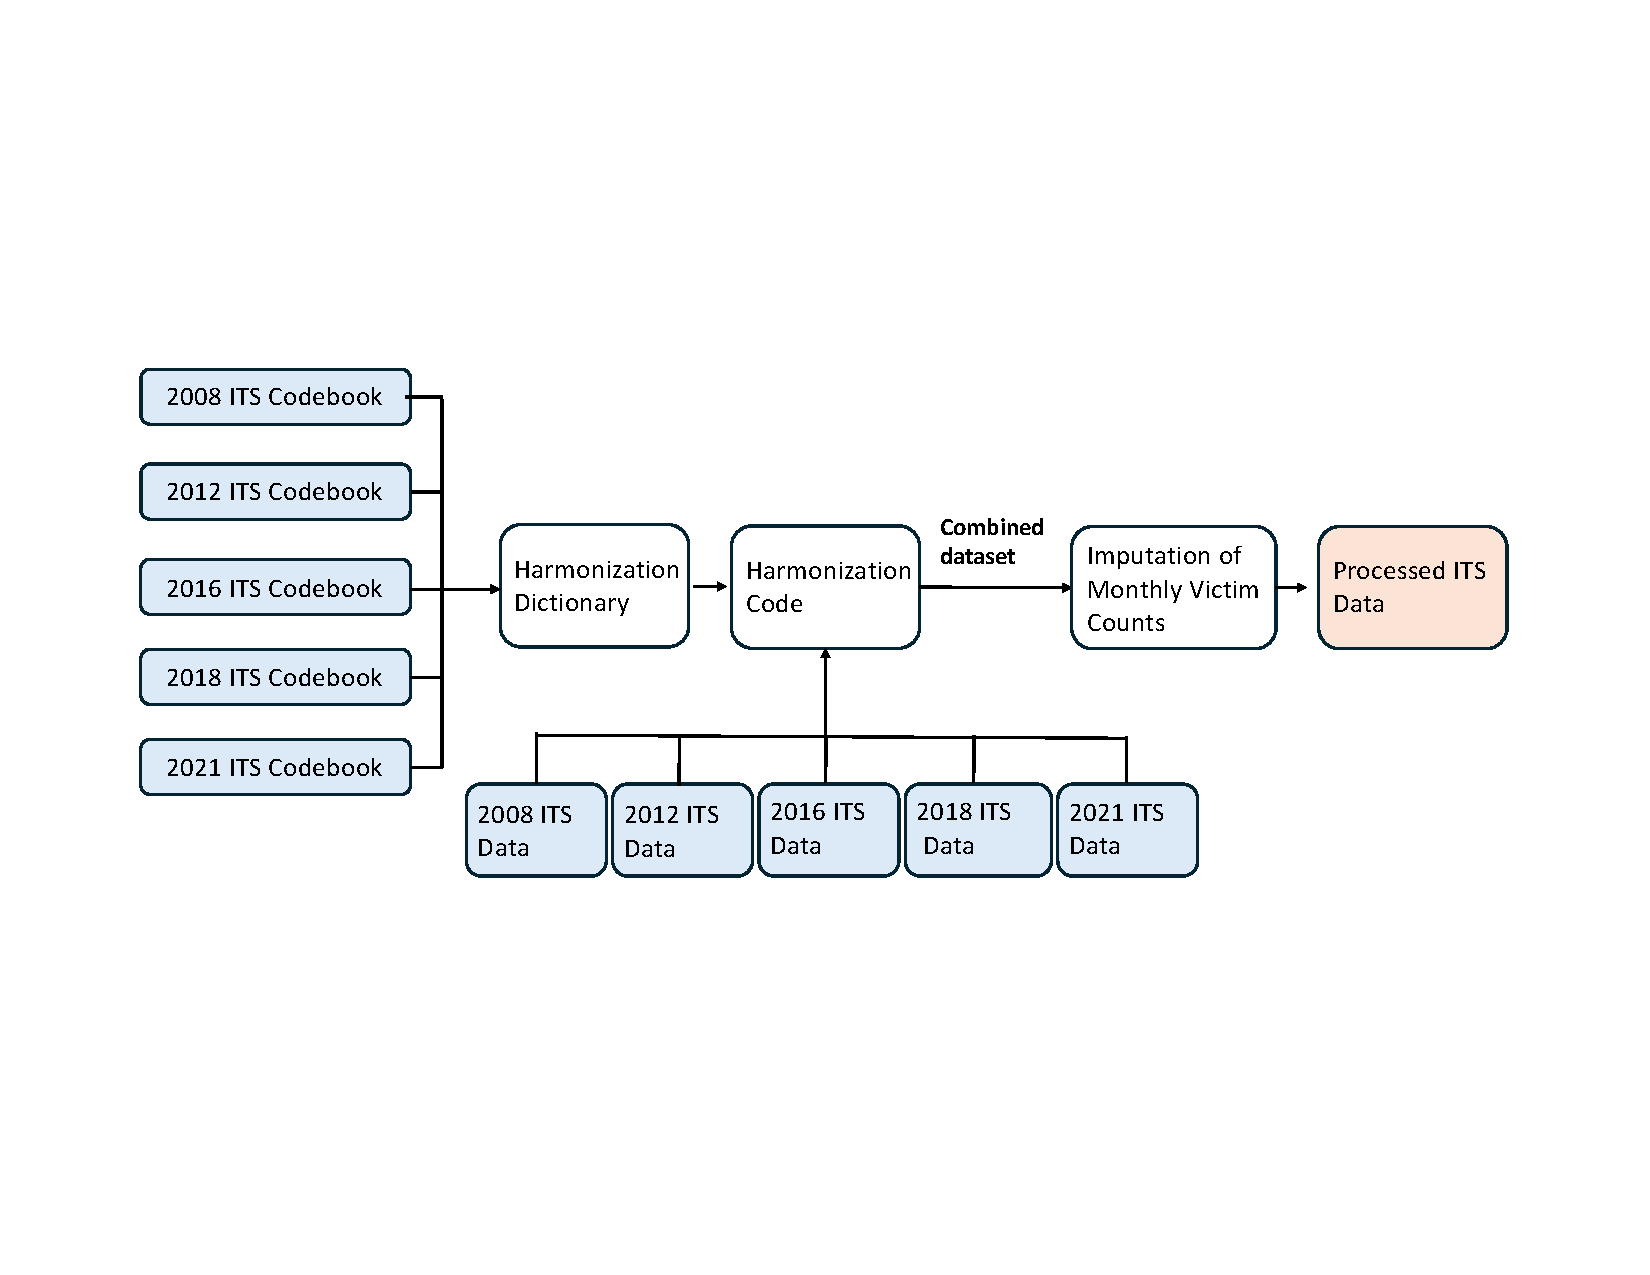
\includegraphics[width=\textwidth, trim={1cm 6cm 1cm 6cm}, clip]{figures/ITS_flowchart.pdf}
    \vspace{-10pt}
    \caption{Workflow for the longitudinal harmonization and processing of the ITS datasets (2008-2021).}
    \label{fig:ITS_processing_flow}
\end{figure}

\subsubsection{Combining the ITS Waves (Harmonization)}
A primary challenge in using these multiple waves is the evolution of the survey over time, which resulted in significant inconsistencies in variable names, value codes, and questions asked over the years, including evolving categories for demographic variables such as household income, and changing variable names and codes for core incident characteristics. Another example of survey inconsistency is that in those administered from 2008 through 2018, the initial screening questions were designed by BJS to identify a broad pool of victims which included individuals who experienced \textit{attempted} IDT (e.g., their credit card was stolen but never used), as well as \textit{successful} IDT (e.g., fraudulent charges were made). Follow-up questions in the survey were then used to differentiate between these two outcomes. In contrast, the 2021 ITS survey was redesigned by BJS to more directly identify victims, and the survey questions focused on whether a respondent's personal information was actually misused for fraudulent purposes. Thus, the 2021 dataset inherently represents a population of successful victims, excluding those who only experienced an attempt.

% \com{Would this fit in the appendix rather than an extended version? If so we might as well include it in the appendix...?} \resp{I can add it in but I think it was the longest part of our old appendix, about 6-7 pages of table mappings}

To address this, we harmonized the data by creating a mapping, or harmonization dictionary, which contained a definitive set of rules for recoding and standardizing variables to ensure that they are conceptually consistent and comparable across all six survey waves. This dictionary was created after careful review and comparison of the codebook associated with each year of the ITS data. For full details of the variable harmonization, recoding schemes, and filtering logic, see the extended version \cite{Anonymous2026SocialCostExtended}. After harmonization, we constructed the final analysis sample by filtering out reported incidents that were ``attempted only,'' resulting in a dataset composed exclusively of victims of successful IDT.
% \rev{Second, we filtered all survey respondents to isolate individuals who reported experiencing at least one type of IDT in the past 12 months. In other words, our final sample only included victims from the past year of the survey.} \com{But I thought this was due to the survey methodology, which only asks whether they had a theft in the past 12mo, not because of our own filtering?} \resp{}
%\com{since these are waves taken every two years, does this mean we only have victims in every other year then...?} \resp{The dataset waves are every 2 years, but the surveys ask questions if the theft occurred in the past year, so it includes data over the year. Also some surveys asked for a specific discovery month and discovery year. For the surveys that didn't ask this, I used the quarter that the survey was administered in to estimate it. More details in Appendix \ref{app:timeline}} 
Since the survey was administered in waves taken approximately every two years, the harmonized dataset only includes victims in every other year. This means that there are ``blackout'' periods in the survey data, which we then mitigated with imputation detailed  in \ref{sec:ITS_impute}.

The application of this harmonization and filtering resulted in a dataset containing a total unweighted sample of 41,091 victims of successful IDT. These victims are distributed across the six survey waves as follows: 2,815 from 2008, 4,401 from 2012, 4,660 from 2014, 10,227 from 2016, 9,928 from 2018, and 9,060 from 2021. 
%\com{Continuing from my previous comment: does this mean that the 4,401 number from 2012 is limited within the 2011-2012 window, while the 4,660 number is limited within the 2013-2014 window, with some months in between with zero counts?} \resp{Yes that is correct. In between the months with zero counts I interpolated the vicitm count so that the data points would connect on the plot.} 
%This combined  sample serves as the basis for our analysis. 
Note that while we used the six survey waves, they are pooled cross-sectional snapshots, not a longitudinal panel of the same individuals. Therefore, we are tracking trends in the population, not the same group of people over 13 years.

To enable generalization of the data findings to the U.S. population, the ITS dataset includes a final survey weight for each respondent. The use of this weight transforms the sample data into nationally representative samples. The weight is calculated by first starting with a base weight that accounts for each household's unequal probability of being selected for the survey. This base weight is then adjusted to account for households that were selected but did not respond, and then calibrated to align the sample's demographic composition with U.S. population totals \cite{ICPSR26362, ICPSR34735, ICPSR36044, ICPSR36829, ICPSR37923, ICPSR38501}. The resulting final weight is given in the dataset and represents a specific number of people in the U.S. population. For example, if a single victim in the dataset has weight 15,000, then their experience is statistically counted as representing 15,000 victims nationwide. {\em Unless otherwise specified, all analyses presented in the rest of this paper utilize data that has been weighted using these final survey weights}. 

\subsubsection{Imputation of Monthly Victim Counts} 
\label{sec:ITS_impute}
Because the ITS survey is administered as a supplement to the NCVS survey with specific reference periods, monthly victim counts are not continuous across the entire 13-year study period (i.e., some months have zero data). To construct a continuous timeline of IDT victimization for comparison against monthly breach data, during the months falling between survey waves where no direct victimization data was collected, we applied a log-linear interpolation. This method assumes a constant rate of change between the observed data points of the adjacent survey waves, allowing us to estimate the victim count during non-survey months and smooth the transitions between the distinct data collection periods.


\subsection{Data Breach Chronology Data}
\label{sec:PRC_processing}

On the exposed data records front, we utilized the Privacy Rights Clearinghouse (PRC) Data Breach Chronology database (Version 2.0) \cite{PRC_Chronology}.  This database catalogs reported data breaches in the United States, providing details like organization profiles, breach types, timelines, and the resulting impact. This raw data was augmented following a multi-stage process to enhance its completeness and accuracy, following similar methods used in \cite{Graves2018Should}. Throughout this section, we use $N$ to denote the total number of data breach incidents and $N_0$ to represent the subset of incidents with undisclosed or missing record counts. Our augmentation process, illustrated in Figure \ref{fig:PRC_processing_flow}, involved the following steps:

\begin{enumerate}
    \item Initial data cleaning following PRC guidelines
    \item Enrichment via federal healthcare disclosures
    \item Estimating national record counts for incidents where only state-level record counts were disclosed
    \item Imputation of record counts for remaining breaches with undisclosed record counts
\end{enumerate}


\begin{figure}[htbp]
    \centering
    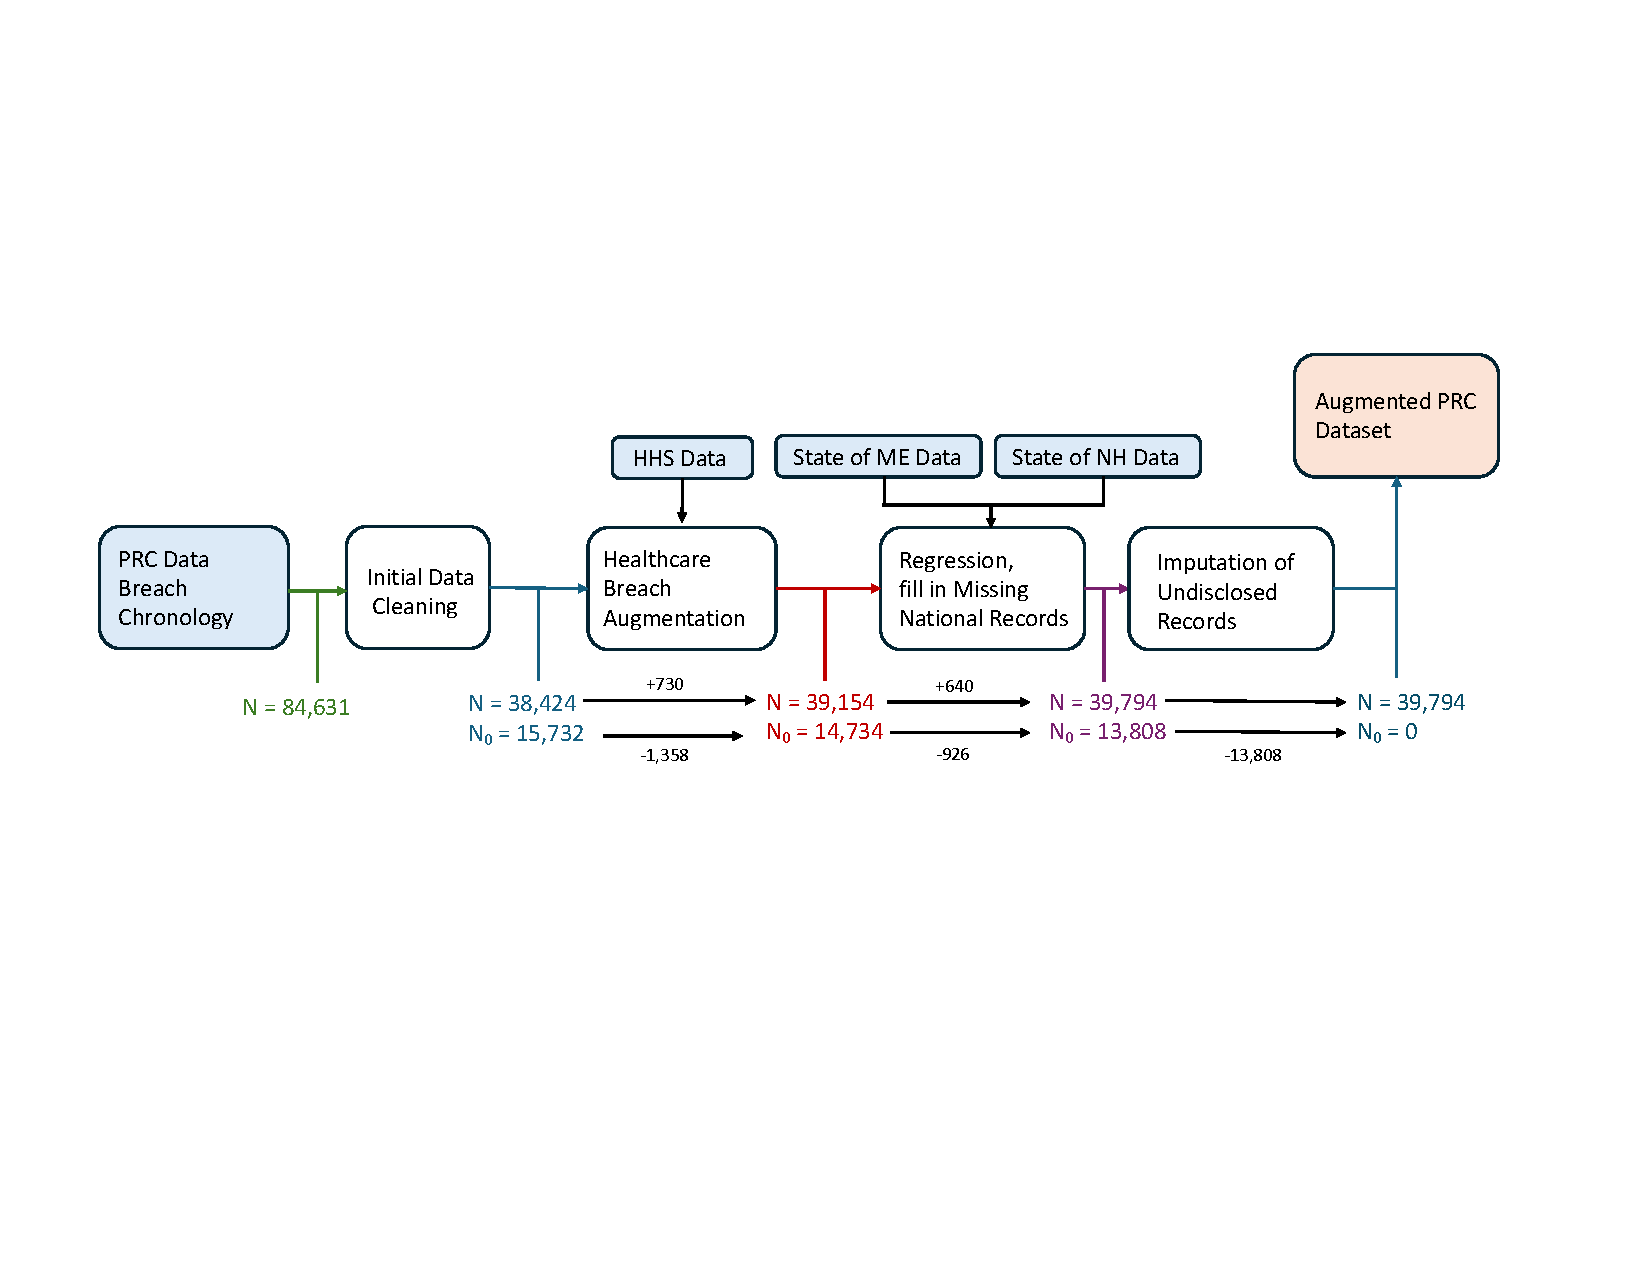
\includegraphics[width=\textwidth, trim={1cm 8.7cm 1cm 6cm}, clip]{figures/PRC_flowchart.pdf}
    \vspace{-10pt}
    \caption{Workflow for the processing and augmentation of the PRC data breach chronology.}
    \label{fig:PRC_processing_flow}
\end{figure}

\subsubsection{Initial Data Cleaning}

To begin, we queried the database for all recorded incidents occurring between 2008 and 2021, specifically extracting the organization name, reported date, and total number of records exposed for each incident. This initial query yielded 84,631 reports. To ensure the integrity of our incident count, we utilized PRC assigned group IDs to consolidate the multiple (state-level) reports stemming from the same underlying event into single observations. This process removed 46,207 duplicate reports, resulting in $N = 38,424$ unique breach events. Of these unique events, $N_0 = 15,732$ initially reported a value of zero for the number of records exposed.


\subsubsection{Integrating Supplemental Healthcare Breach Disclosures}
Following the methodology established by Graves et al. in 2018 \cite{Graves2018Should}, we supplemented the PRC dataset to address missing record counts and incorporate missing events. To improve the coverage of healthcare-related incidents, we cross-referenced the PRC dataset with breach reports from the U.S. Department of Health and Human Services (HHS) \cite{HHS_BreachPortal}. These additions were done in three distinct stages:

\begin{enumerate}[label=(\alph*)]
    \item We first identified and integrated 730 HHS-reported breaches that were entirely absent from the original PRC database, leading to $N = 39,154$. 
    \item For incidents present in both datasets where magnitude values differed, we retained the higher reported value to ensure the capture of the maximum potential impact. There were 7,372 such instances.
    \item Finally, for incidents present in both datasets where PRC originally reported zero or undisclosed record counts, we utilized the HHS data to populate these missing values. Through this process, we successfully recovered 1,358 previously missing magnitude values, thus reducing the data sparsity for healthcare related breaches, and leaving us with $N_0 = 14,734$. 
\end{enumerate}


% First, we integrated any HHS-reported breaches that were absent from the original PRC database. Second, for incidents already present in the PRC dataset but lacking a recorded number of exposed records, we used the HHS data to populate these missing values. \com{What happens when there is magnitude values in both datasets but they differ?} \rev{In the 7,372 instances where magnitude values were present in both datasets but differed, we retained the higher reported value to ensure the capture of the maximum potential impact.} \rev{Beyond these corrections,}, we successfully recovered 1,358 \rev{previously undisclosed magnitude values for incidents where PRC originally reported zero records}, 

% Furthermore, the number of records exposed for major breaches were \rev{manually audited and validated using additional reporting sources}, detailed in \ref{app:PRC_data}. \com{The table in \ref{app:PRC_data} represents only a subset, correct? since the number of mega-breaches is around 20?}

\subsubsection{Regression Modeling Using State-Level Records}
To further recover missing record counts, we used a linear regression model to estimate national exposure from state-level data. Following the approach of \cite{Graves2018Should}, we gathered breach filings from state Attorneys General in Maine and New Hampshire. We selected these states because they consistently report the number of affected residents within their jurisdictions and provide comprehensive data coverage for our study period (2008-2021) \cite{NH_DOJ_Breach, Maine_AG_Breach}. We pooled these two state-level sources and deduplicated the records, prioritizing the highest reported victim count for each incident \cite{NH_DOJ_Breach, Maine_AG_Breach}. To minimize the inclusion of purely local incidents, we filtered out organizations containing keywords indicative of limited geographic scope (e.g. ``Town of'', ``plumbing'', ``electric'', ``dealership'', ``restaurant''). Following this filtration, we pooled the data from both Maine and New Hampshire. In the rare instances where a single breach event was reported in both states (there were only 4 such cases), we retained the observation with the higher reported victim count to avoid double-counting while capturing the upper-bound of the state-level impact. Through this process, we integrated breaches previously absent from the PRC database resulting in a pool of 2,298 unique national-level incidents identified from state-level filings. Of these 2,298, 1,372 were entirely absent from the original PRC database, and 640 were missing from the PRC database augmented with healthcare disclosures. Consequently, we added these 640 new incidents to our augmented dataset, resulting in $N = 39,794$. The remaining 926 incidents were present in the PRC but lacked an associated record count.
%\com{Were all these 2,298 originally missing from PRC, or were some in PRC just missing record count? If the latter we should specify both types}
%\resp{I added a line to clarify this.}
To estimate national impact from these state-level numbers, we used Ordinary Least Squares (OLS) regression to determine the national weight of a single state-level victim. In this model, the independent variable $X$ represents the number of residents impacted within a specific state jurisdiction, while the dependent variable $Y$ represents the total national record exposure for the same incident, obtained from the PRC data. Before running the model, we filtered the data for high-confidence identity matches and verified that the national total number of people affected was at least five times greater than or equal to the state sample of affected residents. This yielded a final sample of 803 unique matched pairs, or incidents where both state-level and national-level data were available. This regression allowed us to recover estimates for these 926 breach events, resulting in $N_0 = 13,808$, and accounting for approximately 121 million records per year.
%\com{Okay, I see that 1,372 were net addition to PRC in incident count, so the other 2,298-1,372=926 incidents were present in PRC but either had 0 record count or some non-zero count which you then revised using the OLS regression?}
%\resp{Yes that's correct, I added a line to clarify that by your first comment above.}

\subsubsection{Imputation of Undisclosed Records}
\label{sec:imputation_of_undisclosed}

Even after the augmentation by two state-level sources,
%After completing the state-level matches, 
we still faced a large volume of 13,808 incidents that lacked an associated number of disclosed records. Again following the methodology of \cite{Graves2018Should}, we sought to find an annual baseline for undisclosed records ($n_u$) through the following three-stage process: 

\begin{enumerate}[label=(\alph*)]
    \item \textit{Weight Calculation:} We categorized each breach in the PRC database by its breach type, and then calculated a typical weight for each category using the known, non-outlier data from the PRC database. These categories from the PRC database were as follows: physical payment card compromises, external cyber attacks, internal threats from authorized users, physical document theft or loss, portable device breaches, stationary device breaches, unintended disclosures, and unknown \cite{PRC_Chronology}. The median value of exposed records for each breach type was used as this weight. Due to the skew of the data, the median was chosen over the mean. 
    
    \item \textit{Baseline Estimation $n_u$:} We define the total undisclosed volume for a specific breach category $j$ as the product of the number of undisclosed incidents $l_j$ and the typical weight (median size) of known breaches in that category $W_j$. The total annual baseline is calculated as follows, where $T$ is the total study duration in years ($T=14$), and $k$ represents the eight PRC breach categories.: $n_u = \frac{1}{T} \sum_{j=1}^k (l_j \times W_j)$. This process allowed us to sum the categorized estimates and led to a finding of an annual $n_u = 1,531,784$ records as a conservative baseline that represents the number of undisclosed exposed records each year.

    \item \textit{Proportional Distribution $R_i$: }We distributed that volume across the zero-count incidents proportionally by year. Specifically, let $I_{u,y}$ be the set of incidents with undisclosed record counts in year $y$, and let $|I_{u,y}|$ be the total number of incidents in such a year. For any incident $i \in I_{u,y}$, the imputed number of records $R_i$ is defined as: $R_i = \frac{n_u}{|I_{u,y}|}$.
\end{enumerate}

The above model could in principle be further refined by separately estimating the baseline for each incident type; see more discussion on this in Section \ref{sec:discussion}.
  In the early years from 2008 to 2011, the number of breaches with undisclosed count $|I_{u,y}|$ was relatively low, averaging around 300 incidents per year. This number steadily increased over the years, reaching 1,109 in 2017. In the most recent years of our study (2018 to 2021), the number of breaches with undisclosed count remained high, consistently exceeding 950 incidents annually and peaking at 1,110 in 2021. The above methodology ensures that the total volume of imputed records in any given year remains constant and equals to $n_u$, thereby preventing the over-inflation of data while still accounting for the cumulative impact of undisclosed breaches. This resulted in a more complete data breach chronology dataset that we used for Section \ref{sec:breach_to_victim}. 

To verify our choice of $n_u$, we compared our estimation against the statistical modeling of the PRC dataset performed by \cite{Edwards2016Hype}. \citet{Edwards2016Hype} identified median breach sizes of 383 records for negligent breaches (when records are exposed accidentally) and 3,141 records for malicious breaches (when records are targeted). Applying these medians to our own dataset provides a quantitative verification of our baseline. Our PRC query identified 13,808 incidents with undisclosed record counts over the 13-year study period following enrichment, averaging approximately 1,062 such incidents per year. If we assume these annual incidents with undisclosed record counts were entirely negligent, the estimated volume would be 406,746 records ($1,062 \times 383$). If they were entirely malicious, the volume would be 3,335,742 records ($1,062 \times 3,141$). Our estimate of $n_u = 1,531,784$ is within this range, approximately 4 times higher than a purely negligent scenario, but significantly lower than a purely malicious one. This alignment suggests that our constant is a middle ground estimate consistent with independent modeling of typical breach magnitudes \cite{Edwards2016Hype}. We recognize that a static annual baseline $n_u$ is a simplification of a likely fluctuating reality. However, this approach provides a stable and conservative lower bound of the undisclosed breach market. Furthermore, because the frequency of incidents with undisclosed record counts $|I_{u,y}|$ increased significantly in later years, a static $n_u$ ensures that the imputed record count per incident remains modest.
%\com{I suppose yet another alternative is to do this for each incident type $j$: $n_u^j=\frac{1}{T}(l_j\times W_j)$, similarly define $i_j$ as incident $i$ of type $j$, belonging to the set $I_{u,y}^j$, the number of incidents of type $j$ in year $u$, such that $|I_{u,y}|=\sum_{j=1}^k |I_{u,y}^j|$, and then finally $R_{i_j}=u_u^j/|I_{u,y}^j|$...?} \resp{I think that is a good idea. But I don't know if we have time to implement this change given that it will likely change our results.. perhaps we can add a paragraph here to mention this alternative, or add it to the discussion?} \com{Yes, if time allows the discussion section would be the right place}
%}